%%%%%%%%%%%%%%%%%%%%%%%%%%%%%%%%%%%%%%%%%
% The Legrand Orange Book
% LaTeX Template
% Version 2.1.1 (14/2/16)
%
% This template has been downloaded from:
% http://www.LaTeXTemplates.com
%
% Original author:
% Mathias Legrand (legrand.mathias@gmail.com) with modifications by:
% Vel (vel@latextemplates.com)
%
% License:
% CC BY-NC-SA 3.0 (http://creativecommons.org/licenses/by-nc-sa/3.0/)
%
% Compiling this template:
% This template uses biber for its bibliography and makeindex for its index.
% When you first open the template, compile it from the command line with the 
% commands below to make sure your LaTeX distribution is configured correctly:
%
% 1) pdflatex main
% 2) makeindex main.idx -s StyleInd.ist
% 3) biber main
% 4) pdflatex main x 2
%
% After this, when you wish to update the bibliography/index use the appropriate
% command above and make sure to compile with pdflatex several times 
% afterwards to propagate your changes to the document.
%
% This template also uses a number of packages which may need to be
% updated to the newest versions for the template to compile. It is strongly
% recommended you update your LaTeX distribution if you have any
% compilation errors.
%
% Important note:
% Chapter heading images should have a 2:1 width:height ratio,
% e.g. 920px width and 460px height.
%
%%%%%%%%%%%%%%%%%%%%%%%%%%%%%%%%%%%%%%%%%

%----------------------------------------------------------------------------------------
%	PACKAGES AND OTHER DOCUMENT CONFIGURATIONS
%----------------------------------------------------------------------------------------

\documentclass[11pt,fleqn]{book} % Default font size and left-justified equations

\usepackage{ifthen} 
\newboolean{VersionProf}
\setboolean{VersionProf}{false}

\usepackage{wasysym}
\usepackage{esint} % various fancy integral symbols
\usepackage{tikz}
\usepackage{tikz-3dplot}
\usepackage{pgfplots}
\pgfplotsset{compat=1.17}
\usetikzlibrary{patterns}
\usepackage{tkz-euclide} 
\usepackage{mathtools}
\usepackage{xurl}
\usepackage[version=4,arrows=pgf-filled,
textfontname=sffamily,
mathfontname=mathsf]{mhchem}
\usepackage{gensymb}
\usepackage{tabularray}
\usepackage{csquotes}
\usepackage{amsmath}
\usepackage{amsfonts}


\usepackage[french]{babel}
\usepackage{dingbat}

\usepackage{environ}
\usepackage{wrapfig}

\NewEnviron{solution}{%
    \ifthenelse{\boolean{VersionProf}}{\begin{solutionA}
        \BODY%*
        \end{solutionA}
    }{%
        \relax%
    }%
}%

\usetikzlibrary {arrows.meta} 

\newcommand{\degC}{{\degree}C}
\newcommand{\dd}{\mathrm{d}}
\newcommand{\div}{\mathrm{div}}
\newcommand{\rot}{\vv{\mathrm{div}}}
\newcommand{\grad}{\vv{\mathrm{grad}}}
\NewCommandCopy{\amshbar}{\hbar}

\tikzset{
    support/.style={
        pattern=north east lines,
        draw=none,
        minimum width=0.3,
        minimum height=0.6
    }
    ,>=latex
}

\usepackage[d]{esvect}

%SPECIFIC TO THIS CHAPTER
\usepackage{physics}
\usepackage{ifthen}
\usepackage[outline]{contour} % glow around text
\usetikzlibrary{calc} % for pic
\usetikzlibrary{angles,quotes} % for pic
\usetikzlibrary{patterns}
\tikzset{>=latex} % for LaTeX arrow head
\contourlength{1.2pt}

\colorlet{myred}{red!65!black}
\definecolor{myred}{RGB}{243,102,25}
\tikzstyle{ground}=[preaction={fill,top color=black!10,bottom color=black!5,shading angle=20},
                    fill,pattern=north east lines,draw=none,minimum width=0.3,minimum height=0.6]
\tikzstyle{mass}=[line width=0.6,myred,fill=myred!40,rounded corners=1,
                  top color=myred!40,bottom color=myred!20,shading angle=20]
\tikzstyle{rope}=[myred!30,line width=1.2,line cap=round] %very thick

% FORCES SWITCH
\tikzstyle{force}=[->,myred,ultra thick,line cap=round]
\tikzstyle{Fproj}=[force,myred!60]
\newboolean{showforces}
\setboolean{showforces}{true}
%----------------------------------------------------------------------------------------

\input{structure} % Insert the commands.tex file which contains the majority of the structure behind the template

\begin{document}

%----------------------------------------------------------------------------------------
%	TABLE OF CONTENTS
%----------------------------------------------------------------------------------------

%\usechapterimagefalse % If you don't want to include a chapter image, use this to toggle images off - it can be enabled later with \usechapterimagetrue

\chapterimage{voile_solaire.png} % Table of contents heading image

%\pagestyle{empty} % No headers

%\tableofcontents % Print the table of contents itself

%\cleardoublepage % Forces the first chapter to start on an odd page so it's on the right

%\pagestyle{fancy} % Print headers again



%\part{\'{E}lectromagnétisme}

\setcounter{chapter}{17}

\chapter{Ondes électromagnétiques et conducteurs}

Dans les chapitrs précédents, nous avons étudié la propagation des ondes lumineuses dans le vide ainsi que dans certains milieux particuliers. Ce chapitre sera consacré à la description des milieux conducteurs, qui interagissent d'une manière particulière avec le champ électromagnétique. En effet, dans un matérieu conducteur, les électrons sont libres de se déplacer, et le champ électromagnétique va les mettre en mouvement, ce qui va en retour agir sur le champ électromagnétique lui-même. 

En raison de leurs propriétés particulières, les conducteurs sont omniprésents dans tous les appareils utilisant des ondes électromagnétiques, tels que les appareils de télécommunications, les four à micro-ondes, les capteurs de lumière... Dans ce chapitre, nous allons montrer en quoi ils pemettent de modifier, et même de guider les ondes électromagnétiques.

\section{Conduction électrique}

On trouve dans la nature des matériaux dits isolants, qui ne peuvent pas conduire l'électricité, et d'autres dits conducteurs. Le caractère isolant ou conducteur d'un matériau est lié à sa structure microscopique : un matériau sera conducteur si les électrons sont libres de circuler, ce qui ne se produit que dans certaines configurations cristallines.

\begin{capex}
	On considère un fil de rayon $r = 0.1$\,mm parcouru par un courant $i = 100$\,mA. On donne la densité d'électrons dans un conducteur $n_e \approx 10^{28}$\,m$^{-3}$. Déterminer la longueur d'onde de De Broglie d'un électron. Conclure quant à la nature quantique ou classique du phénomène de conduction électrique.
\end{capex}

\begin{remark}
	La raison pour laquelle certains matériaux conduisent l'électricité et d'autres non est quantique : il faut que les états quantiques accessibles par les électrons soient tels que leurs vitesses ne se compensent pas. Dans un matériau non conducteur ou semiconducteur, il y a des électrons qui se déplacent, mais ils occupent des états quantiques bien définis pour lesquels les vitesses se compensent. 
\end{remark}

\subsection{Loi d'Ohm locale}

Nous n'allons pas décrire le phénomène de conduction électrique de manière quantique (cela nécessite des notions de physique du solide que vous verrez en L3 ou en M1 si vous continuez à faire de la physique). Nous allons plutôt utiliser une loi phénoménologique qui décrit le phénomène de conduction. Nous connaissons déjà la loi d'Ohm $U = R I$ qui relie la tension aux bornes d'une résistance et le courant qui la traverse. La loi d'Ohm locale traduit le même phénomène à l'échelle microscopique, et tire parti du fait que $U$ est proportionnelle au champ électrique dans la résistance, alors que $I$ est proportionnelle à la densité volumique de courant.

\begin{capex}
	Faire une analogie formelle entre la loi d'Ohm et la notion de résistance thermique. Proposer alors une loi empirique locale, analogue à la loi de Fourier, pour la conduction électrique.
\end{capex}

\begin{theorem}[Loi d'Ohm locale]
	Dans un conducteur, la densité volumique de courant $\vv j$ et le champ électrique $\vv E$ sont reliés par la relation suivante :
	\begin{equation}
		\vv j = \gamma \vv E
	\end{equation}
	où $\gamma$ est appelée la conductivité électrique du milieu. Elle se mesure en S$\cdot$m$^{-1}$.
\end{theorem}

\paragraph*{Le modèle de Drude}

	Il est possible de retrouver cette formule à partir d'un modèle simpliste de la conduction, appelé "modèle de Drude". Ce modèle utilise cependant des hypothèses qui ne sont absolument pas vérifiées : il suppose que les électrons ont un comportement classique (et non pas quantique), et par ailleurs modélise l'interaction des électrons avec le réseau cristallin du métal comme une force de frottement fluide alors qu'il s'agit en réalité d'une interaction de nature électrostatique.

\begin{figure}[htbp]
	\centering 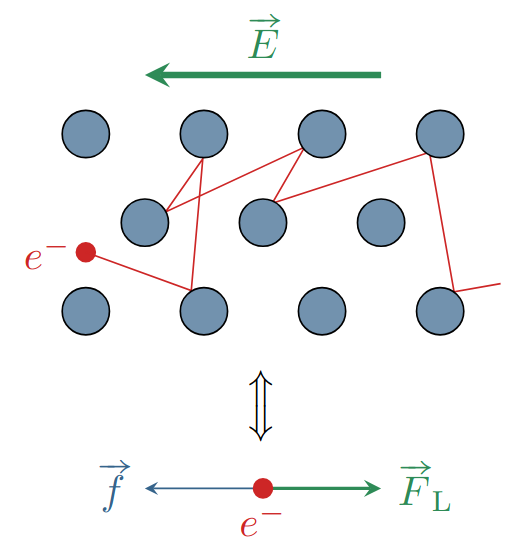
\includegraphics[width=0.3\linewidth]{drude.png}
	\caption{Principe du modèle de Drude. Dans ce modèle, on suppose (à tort) que les électrons ont un comportement classique, et qu'ils sont soumis à la force de Lorentz électrique $\vv{F_L}$ ainsi qu'une force de frottement fluide $\vv f$ qui modélise des collisions avec les ions du réseau cristallin se faisant avec un temps caractéristique $\tau$. Source : poly de cours de Etienne Thibierge.}
\end{figure}

	Dans ce modèle, les électrons sont soumis à un champ électrique $\vv E$. Comme ils sont non relativistes, on peut montrer que la composante électrique de la force de Lorentz domine devant la composante magnétique (cf cours sur les ondes dans les plasmas). On suppose par ailleurs que les interactions entre les électrons et les ions du réseau peuvent se modéliser par une force de frottement fluide $\vv{F_f} = - \dfrac{m_e}{\tau} \vv v$ où $\vv v$ est la vitesse des électrons et $\tau$ est un temps caractéristique de collision avec les ions du réseau. Ainsi :
	\begin{equation}
		m_e \frac{\dd \vv v}{\dd t} = - e \vv E - \dfrac{m_e}{\tau} \vv v
	\end{equation}
	En régime permanent, nous obtenons $\vv v = - \dfrac{e \tau}{m_e} \vv E$ et donc, en utilisant $\vv j = - n e \vv v$ :
	\begin{equation}
		\vv j = \frac{n e^2 \tau}{m_e} \vv E
	\end{equation}
	On retrouve ainsi la loi d'Ohm avec une conductivité $\gamma = \frac{n e^2 \tau}{m_e}$.	Ce modèle est tellement classique qu'il est bon de savoir calculer la conductivité électrique dans ce cadre. Néanmoins, toute application numérique montrera que le modèle ne fonctionne pas du tout, et en particulier il est incapable d'expliquer pourquoi la conductivité électrique varie avec des ordres de grandeur d'écart selon les matériaux.

\subsubsection{Electroneutralité du conducteur}

La conservation de la charge dans un conducteur impose :
\begin{equation}
	\frac{\partial \rho}{\partial t} + \div \vv j = 0
\end{equation}
En combinant avec la loi d'Ohm $\vv j = \gamma \vv E$ et l'équation de Maxwell-Gauss, nous obtenons :
\begin{equation}
	\frac{\partial \rho}{\partial t} + \frac{\rho}{\tau_c} = 0
\end{equation}
où $\tau_c = \frac{\epsilon_0}{\gamma} \approx 10^{-19}$\,s. Ainsi la densité volumiques de charges décroît exponentiellement dans le conducteur avec un temps caractéristique $\tau_c$ très court, qui est négligeable devant la période de la plupart des ondes électromagnétiques utilisées habituellement. On pourra donc considérer que les conducteurs sont électriquement neutres :

\begin{proposition}[Electroneutralité des conducteurs]
	La densité volumique de charges $\rho$ est généralement nulle dans un conducteur électrique, sauf lorsque l'on travaille à très haute fréquence.
\end{proposition}

\subsection{Bilan d'énergie dans une résistance}

Nous pouvons désormais faire un bilan énergétique sur un matériau conducteur :
\begin{capex}
	On considère une résistance électrique de section $S$ et de longueur $L$. Déterminer l'expression de la résistance en fonction de $S, L$ et la conductivité $\gamma$ du milieu. Réaliser un bilan énergétique dans la résistance et retrouver ainsi l'expression de la puissance dissipée par effet Joule dans la résistance.
\end{capex}

\begin{figure}[htbp]
	\centering 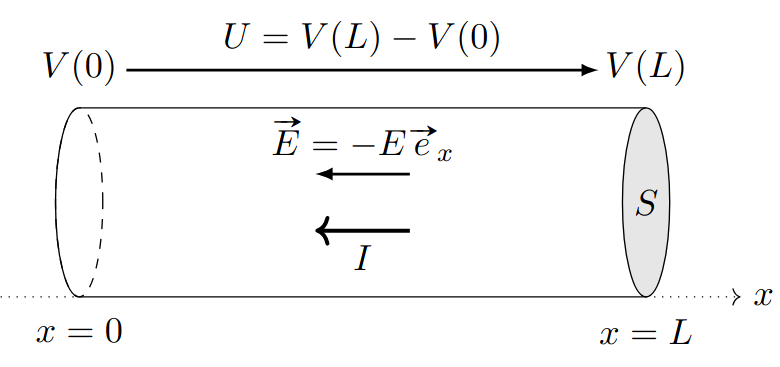
\includegraphics[width=0.5\linewidth]{schema_resistance.png}
	\caption{Schéma d'un matériau conducteur cylindrique dont on souhaite calculer la résistance. Source : poly de cours de Maxime Champion.}
\end{figure}

Nous en déduisons la propriété suivante, à connaître :
\begin{proposition}
	Considérons un élément conducteur, de conductivité $\gamma$, parcouru par un courant. On note $e$ sa longueur dans le sens du courant, et $S$ sa section, prise perpendiculairement au sens du courant. Alors le matériau est équivalent à une résistance électrique de valeur :
	\begin{equation}
		R = \frac{e}{\gamma S}
	\end{equation}
\end{proposition}

\subsection{Conductivité complexe en régime sinusoïdal}

La notion de conductivité peut être élargie à des matériaux autres que les matériaux conducteurs, notamment en régime sinusoïdal forcé. L'étude harmonique a en effet du sens dans le cadre de l'étude d'ondes électromagnétiques, pour lesquelles toutes les quantités dépendent sinusoïdalement du temps. C'est le cas notamment si l'on adopte le cadre du modèle de Drude, en régime sinusoïdal forcé nous pouvons écrire :
\begin{equation}
	i \omega m_e \underline{\vv v} = - \frac{m_e}{\tau} \underline{\vv v} - e \underline{\vv E}
\end{equation}
Les étapes suivantes sont similaires et nous pouvons conclure que :
\begin{equation}
	\underline{\vv j} = \underline{\gamma} \underline{\vv E}
\end{equation}
où
\begin{equation}
	\underline{\gamma} = \frac{n e^2 \tau}{m_e} \frac{1}{1 + i \omega \tau}
\end{equation}
Autrement dit, la conductivité électrique du milieu diminue lorsque la fréquence augmente, en raison notamment de l'inertie des électrons qui n'ont pas le temps d'être entrainés par le champ électrique au cours d'une période.

Bien entendu, l'expression obtenue par le modèle de Drude n'est pas satisfaisante pour décrire les observations expérimentales, puisqu'elle est fondée sur un modèle classique dont les conditions de validité ne sont pas vérifiées, un calcul correct de la conductivité complexe du milieu doit faire intervenir un modèle quantique.

On peut cependant définir la conductivité complexe pour d'autres matériaux, et notamment pour les plasmas.
\begin{capex}
	Montrer qu'en régime sinusoïdal forcé, un plasma peut être décrit par une loi d'Ohm locale complexe. Déterminer la condcutivité électrique complexe du plasma.
\end{capex}

\section{Propagation des ondes électromagnétiques dans un conducteur}

\subsection{Approximation des régimes quasi stationnaires}

Dans les conducteurs, on pourra souvent faire des hypothèses simplificatrices sur la propagation du champ électromagnétique. Parmi ces hypothèses, on peut en particulier réaliser l'approximation des régimes quasi stationnaires, qui permet de retrouver les lois de l'électricité.

\subsubsection{Définition}

\begin{definition}
	Dans le cadre de l’approximation des régimes quasi-stationnaires (ARQS), on suppose que le temps caractéristique nécessaire aux ondes électromagnétiques pour parcourir la taille caractéristique du système $L$ est très rapide devant le temps caractéristique $T$ des phénomènes étudiés, soit $L \ll cT$.

	Ceci revient à supposer que la propagation des ondes électromagnétiques est instantanée.
\end{definition}

Cette hypothèse permet de négliger tous les termes de propagation dans les équations de Maxwell. Dans un circuit électrique de TP, dont la taille fait environ 1\,m, l'ARQS sera vérifiée tant que $T \gg L/c$. Cette approximation est bien vérifiée pour des fréquences allant jusqu'à 1\,MHz.

On admet la propriété suivante :
\begin{proposition}
	Dans le cadre de l'ARQS, et lorsque la densité volumique de charge $\rho$ est faible ($\rho \ll ||\vv j||/c$), on peut négliger le terme de courant de déplacement dans l'équation de Maxwell-Ampère, ainsi que la dérivée temporelle dans l'équation de conservation de la charge. On parle d'ARQS magnétique.

	On a ainsi $\vv rot \vv B = \mu_0 \vv j$ et $\div \vv j = 0$.
\end{proposition}

\begin{remark}
	La condition $\rho \ll ||\vv j||/c$ est généralement vérifiée dans les conducteurs puisqu'ils sont électriquement neutres ($\rho = 0$). Une exception notable est le cas du condensateur en régime variable.
\end{remark}

\subsubsection{Loi des noeuds}

Une des conséquences de l'ARQS magnétique est la loi des noeuds. Considérons une intersection entre des fils électriques. Nous définissons une surface fermée $\Sigma$ contenant le noeud électrique. Cette surface coupe les fils, en formant des sections notées $\vv{S_i}$, où le vecteur $\vv{S_i}$ correspond au fil $i$ et est orienté parallèlement au fil, dans le sens sortant de la surface $\Sigma$. Alors la somme des courants entrants vers le noeuds s'écrit :
\begin{equation}
	I_{\rm entrant}  = - \sum_i \vv \vv{j_i} S_i = - \oiint_\Sigma \vv j \cdot \vv{\dd S}
\end{equation}
Or, la forme intégrale de la conservation de la charge nous permet d'écrire que :
\begin{equation}
	\frac{\dd Q_{\rm int}}{\dd t} + \oiint_\Sigma \vv j \cdot \vv{\dd S} = 0
\end{equation}
La dérivée temporelle pouvant être considérée comme nulle dans le cadre de l'ARQS, nous concluons que :
\begin{equation}
	I_{\rm entrant} = 0
\end{equation}
ce qui correspond à la loi des noeuds.

\begin{figure}[htbp]
	\centering 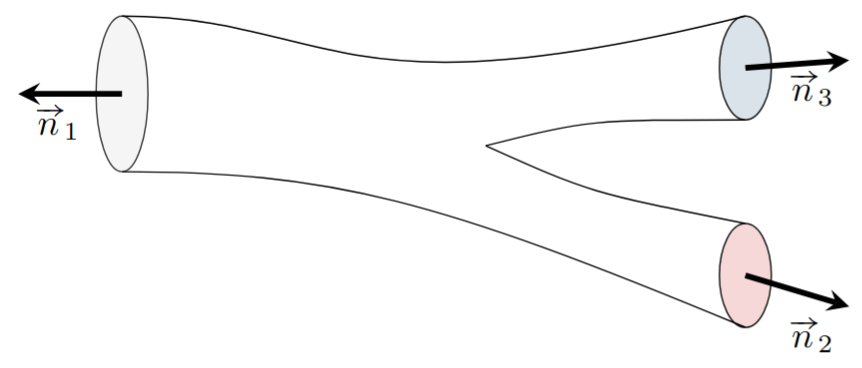
\includegraphics[width=0.5\linewidth]{loi_des_noeuds.png}
	\caption{Schéma d'un noeud électrique auquel on applique la forme intégrale de la conservation de la charge. Source : poly de cours de Maxime Champion.}
\end{figure}

\subsubsection{Loi des mailles}

La loi des mailles peut également s'obtenir, cette fois-ci en l'absence de phénomènes d'induction. Considérons un circuit électrique fermé, correspondant à un contour $\Gamma$. Par définition, la force électromotrice $e$ le long de ce circuit est la circulation du champ électrique le long de ce contour, qui est définie comme :
\begin{equation}
	e = \oint_\Gamma \vv E \cdot \vv{\dd \ell}
\end{equation}
Nous appliquons la loi de Faraday à ce circuit :
\begin{equation}
	e = - \frac{\dd \Phi}{\dd t} = 0
\end{equation}
où $\Phi$ est le flux du champ magnétique à travers le circuit. En l'absence de champ magnétique, ou pour un champ lentement variable, nous en concluons directement que $e=0$, c'est-à-dire que la somme des tensions aux bornes de chaque dipôle s'annule, ce qui correspond à la loi des mailles.

\subsection{Réflexion d'une onde sur un conducteur, effet de peau}

Que se passe-t-il lorsqu'une onde électromagnétique, initialement dans le vide, rencontre un matériau conducteur ? On s'attend à avoir une équation d'onde différente de celle du vide, en particulier nous savons déjà que si une onde se propage dans le conducteur :
\begin{itemize}
	\item Les électrons présents dans le conducteur vont affecter la propagation de l'onde ce qui, comme pour le plasma, va modifier l'équation d'onde et la relation de dispersion ;
	\item De l'énergie va être dissipée par effet Joule, ce qui va modifier le bilan énergétique de l'onde.
\end{itemize}

\begin{capex}
	Etablir l'équation de propagation du champ électromagnétique dans un conducteur de conductivité $\gamma$. Quel est le nom de cette équation ? En déduire la relation de dispersion d'une onde plane progressive harmonique.  
\end{capex}

\begin{figure}[htbp]
	\centering 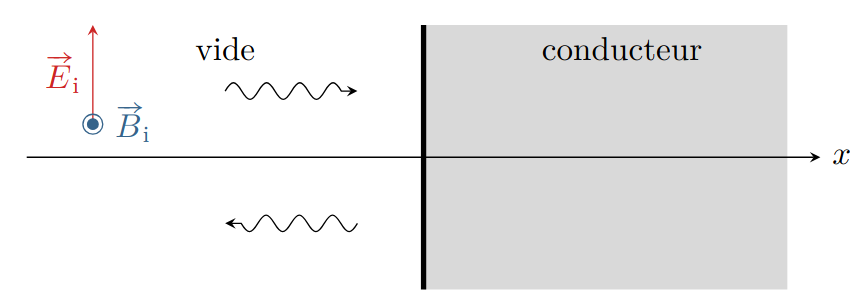
\includegraphics[width=0.5\linewidth]{reflexion.png}
	\caption{Onde électromagnétique incidente sur un conducteur. Source : poly de cours de Maxime Champion.}
\end{figure}

Pour comprendre la structure d'une onde, on s'intéresse à une onde plane progressive monochromatique polarisée rectilignement selon $\vv{e_x}$, en incidence normale sur un conducteur parfait, occupant le demi-espace $z>0$. On adopte la représentation complexe :
\begin{equation}
	\underline{\vv E_i} = E_0 e^{i(\omega t - k_i z)} \vv{e_x}
\end{equation}
L'onde incidente va donner naissance à une onde réfléchie, notée $\underline{\vv{E_r}}$ et à une onde transmise dans le métal, notée $\underline{\vv{E_t}}$. L'onde réfléchie se propage dans le sens des $z$ décroissants, et l'onde transmise dans le sens des $z$ croissants, on supposera ainsi qu'elles prennent la forme suivante :
\begin{align}
	\underline{\vv E_r} &= \underline{E}_r e^{i(\omega t + k_r z)} \vv{e_x} \\ 
	\underline{\vv E_t} &= \underline{E}_t e^{i(\omega t - k_t z)} \vv{e_x} 
\end{align}

\begin{capex}
	Justifier la forme proposée pour les ondes réfléchie et transmise et les représenter sur le schéma. Déterminer le champ magnétique associé à chacune des deux ondes. En exploitant les relations de dispersion dans le vide et dans le conducteur, et la continuité du champ électromagnétique à l'interface, déterminer l'expression de $k_r$ et $k_t$. Interpréter la forme de l'onde transmise.
\end{capex}

On obtient alors une onde transmise de la forme :
\begin{equation}
	\underline{\vv E_t} = \underline{E}_t \cos\left(\omega t - \frac{z}{\delta}\right) e^{-z/\delta}
\end{equation}
où l'on définit l'épaisseur de peau :
\begin{definition}
	L'épaisseur de peau, $\delta = \sqrt{\dfrac{2}{\mu_0 \gamma \omega}}$, est la profondeur de pénétration d'une onde électromagnétique dans un conducteur. Elle dépend de la pulsation $\omega$ de l'onde. 
\end{definition}
On constate qu'une onde électromagnétique ne peut pas pénétrer profondément dans un milieu conducteur, et ce d'autant plus que la conductivité du milieu et la fréquence de l'onde sont élevées.

\begin{figure}[htbp]
	\centering 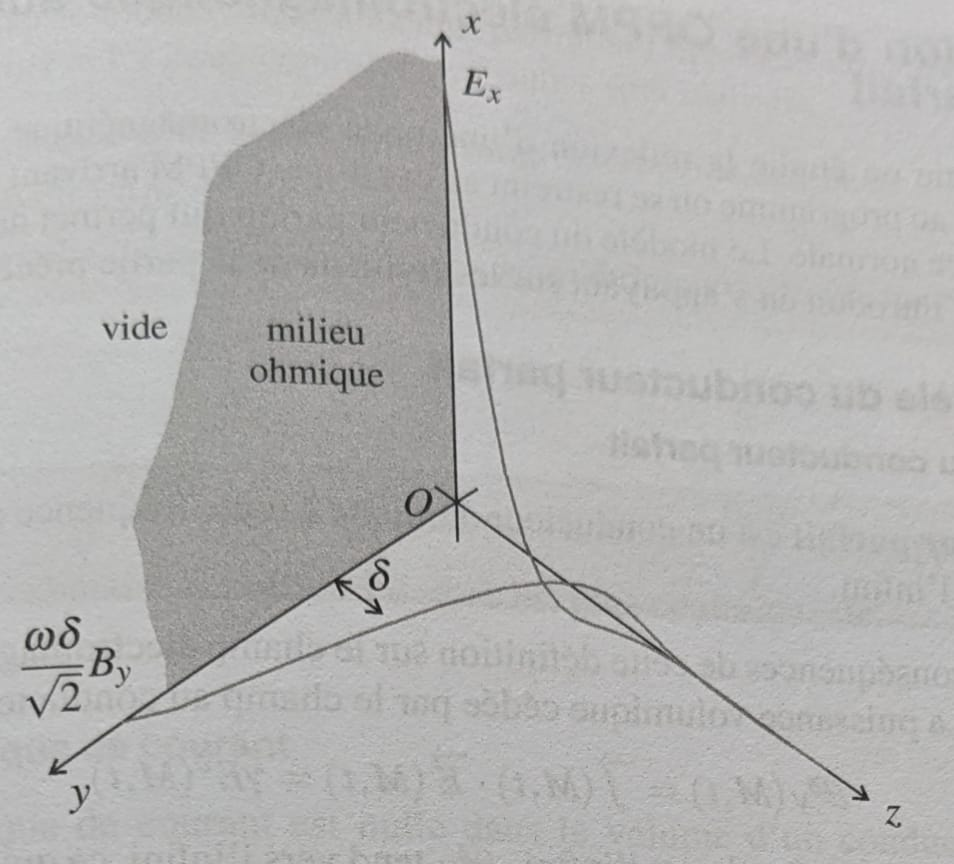
\includegraphics[width=0.6\linewidth]{effet_de_peau.jpeg}
	\caption{Schéma du champ électrique et magnétique dans le conducteur à un instant donné : l'épaisseur de peau est du même ordre de grandeur que la longueur d'onde de l'onde dans le conducteur. Source : Vuibert et al.(2025), \textit{Tout-en-Un MP/MP}$^\ast$, Dunod.}
\end{figure}

%\begin{capex}
%	Calculer le vecteur de Poynting des ondes incidente, réfléchie et transmise. Définir le coefficient de réflexion en énergie de l'onde. Montrer que l'intégralité de l'énergie transmise vers le conducteur est dissipée par effet Joule.
%\end{capex}

\section{Conducteur parfait}

Nous avons vu que dans les conducteurs, les ondes électromagnétiques ne peuvent pas pénétrer avec une profondeur trop importante : le conducteur électromagnétique fait écran à la propagation de l'onde. Il est possible de simplifier ce modèle en considérant le cas limite du conducteur parfait : dans ce cas, la conductivité tend vers l'infini, si bien que l'épaisseur de peau tend vers zéro :
\begin{definition}[Modèle du conducteur parfait]
	On dit qu'un conducteur est parfait lorsque sa conductivité $\gamma$ tend vers l'infini. Dans ce cas, aucun champ électrique ne peux exister au sein du conducteur. Dans une situation indépendante du temps, on peut ainsi considérer que l'ensembple du volume conducteur est au même potentiel électrique $V$.
\end{definition}

\subsection{Notion de courant surfacique}

Dans le cadre du modèle du conducteur parfait, on peut avoir une discontinuité de champ électrique et/ou magnétique à la surface du conducteur. Cette discontinuité s'accompagne de la présence de charges et de courants à la surface. Prenons l'exemple de l'onde en incidence normale sur un conducteur vu précédemment. La densité volumique de courants dans le conducteur se calcule à partir de l'équation de Maxwell-Ampère :
\begin{align}
	\underline{\vv j} &= \frac{1}{\mu_0} \rot(\underline{\vv B}) \\
	&= \frac{1}{\mu_0} \frac{E_0(1+i)}{i \delta \omega} \frac{\partial}{\partial z} \left[ e^{i(\omega t - \frac{z}{\delta})}  e^{-z/\delta} \right] \vv{e_x} \\
	&= \frac{1}{\mu_0} \frac{E_0(1+i)^2}{i \delta^2 \omega}  e^{i(\omega t - \frac{z}{\delta})}  e^{-z/\delta}  \vv{e_x} \\
	&= \frac{1}{\mu_0} \frac{2 E_0}{\delta^2 \omega}  e^{i(\omega t - \frac{z}{\delta})}  e^{-z/\delta} \vv{e_x}
\end{align}
Ces courants forment une nappe d'épaisseur $\delta$. Lorsque $\delta \to 0$, l'épaisseur de la nappe de courants tend vers 0 mais l'amplitude de la densité volumique de courant diverge ! Cela ne pose pas de problème physique puisque la quantité totale de courant transportée dans l'interface reste finie, et on peut alors définir le courant surfacique :
\begin{definition}[Courant surfacique]
	Un courant surfacique, noté $\vv{j_s}$, est un courant qui parcourt une surface. Il se mesure en A$\cdot$m$^{-1}$. $\vv{j_s}$ est orienté dans le sens du courant, et sa norme est telle que $\dd I = ||\vv{j_s}|| \dd \ell$ est le courant élémentaire qui traverse un segment de longueur $\dd \ell$ perpendiculaire à $\vv{j_s}$.
	On peut passer de la densité volumique à la densité surfacique de courant selon la loi :
	\begin{equation}
		\vv{j_s} = \int_0^e \vv j \dd z
	\end{equation}
	où l'on intègre sur une couche d'épaisseur $e$ selon la coordonnée $z$ orientée perpendiculairement à la surface considérée.
\end{definition}

\begin{figure}[htbp]
	\centering 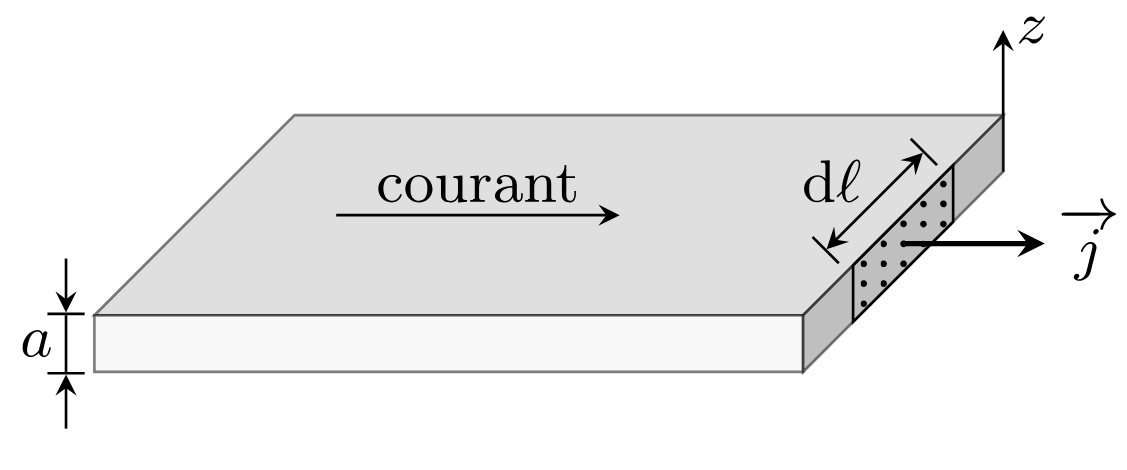
\includegraphics[width=0.5\linewidth]{courant_surfacique.png}
	\caption{Nappe de courant pouvant être décrite par une densité surfacique de courant. Source : femto-physique.fr}
\end{figure}

Dans notre cas, la densité surfacique de courant s'écrit :
\begin{equation}
	\underline{\vv j_s} = \int_0^\infty \underline{\vv j} \dd z = \frac{1}{\mu_0} \frac{2 E_0}{\delta^2 \omega} \times \frac{\delta}{(1+i)} e^{i\omega t} \vv{e_x} 
\end{equation}
Autrement dit, en repassant en réels, avec $1 + i = \sqrt{2} e^{i\frac{\pi}{4}}$, on obtient :
\begin{equation}
	\vv j_s = \sqrt{2} \frac{E_0}{\mu_0 \delta \omega} \cos\left(\omega t - \frac{\pi}{4}\right) \vv{e_x}
\end{equation}
Nous constatons alors que cette expression est reliée à la différence de champ magnétique observée entre le conducteur et le vide :
\begin{equation}
	\vv B(z=0^+) - \vv B(z = 0^-) = \mu_0 \vv{j_s} \wedge \vv{e_z}
\end{equation}

\subsection{Relations de passage}

Dans le cas de l'onde en incidence normale, polarisée rectilignement, nous avons pu démontrer une relation entre la discontinuité du champ magnétique à l'interface et le courant surfacique. Ce type de propriété se généralise à tous les conducteurs parfaits, et des propriétés similaires existent pour le champ électrique :
\begin{theorem}[Relations de passage]
	Considérons une interface entre deux milieux 1 et 2, de normale $\vv n_{1 \to 2}$. Les champs de part et d'autre de l'interface sont reliés par les relations suivantes :
	\begin{equation}
		\begin{dcases}
			\vv E_2 - \vv E_1 = \dfrac{\sigma}{\epsilon_0} \vv n_{1\to 2} \\
			\vv B_2 - \vv B_1 = \mu_0 \vv{j_s} \wedge \vv n{1\to 2}
		\end{dcases}
	\end{equation}
	où $\sigma$ est la densité surfacique de charge à l'interface, et $\vv{j_s}$ est le courant surfacique à l'interface.
	En particulier, il y a \textbf{continuité de la composante tangentielle du champ électrique et de la composante normale du champ magnétique} à l'interface.
\end{theorem}

\begin{figure}[htbp]
	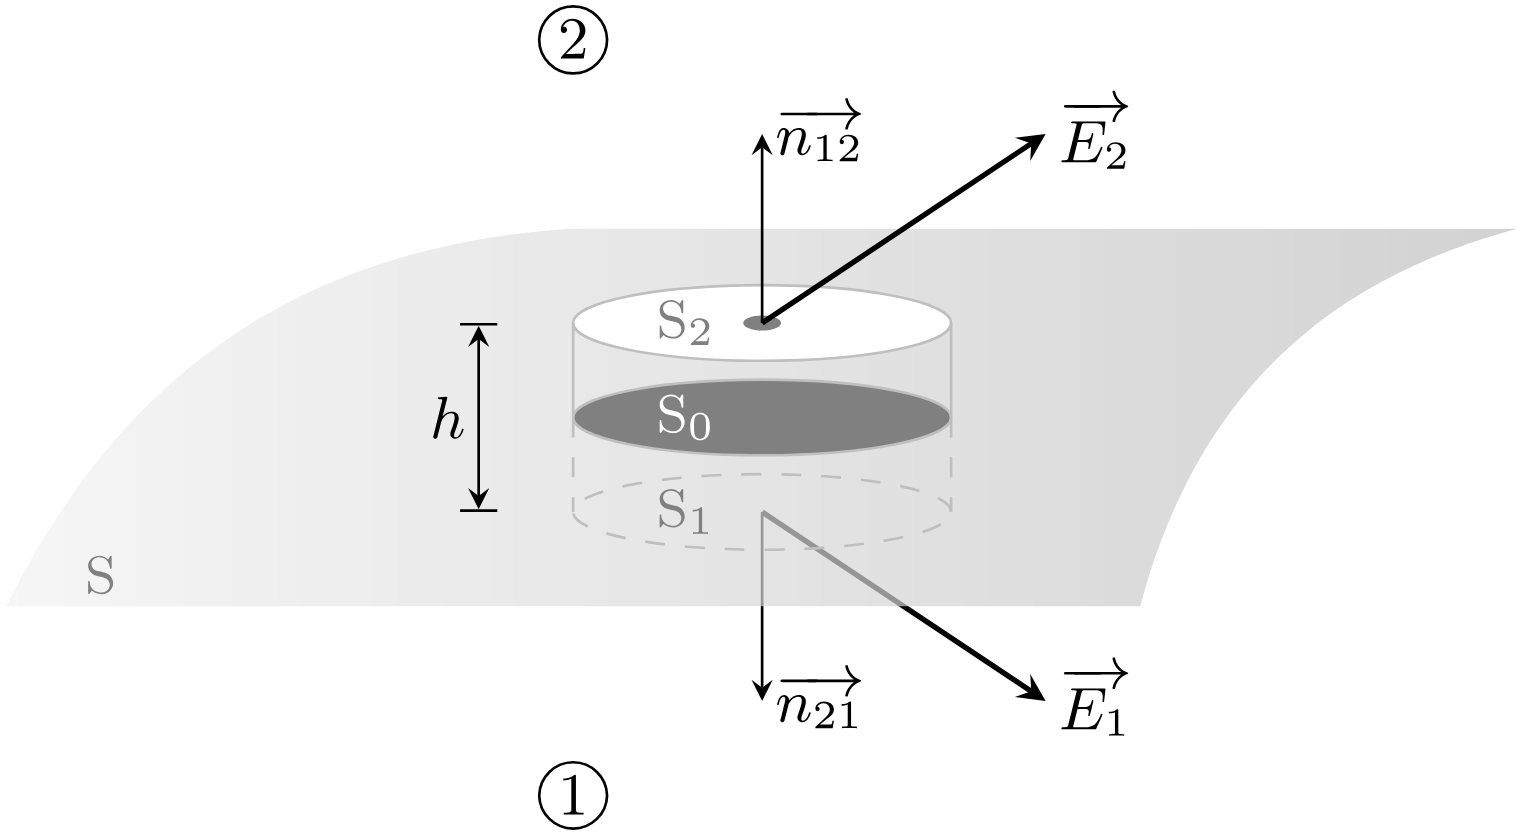
\includegraphics[width=0.36\linewidth]{passage_E_normal.png}
	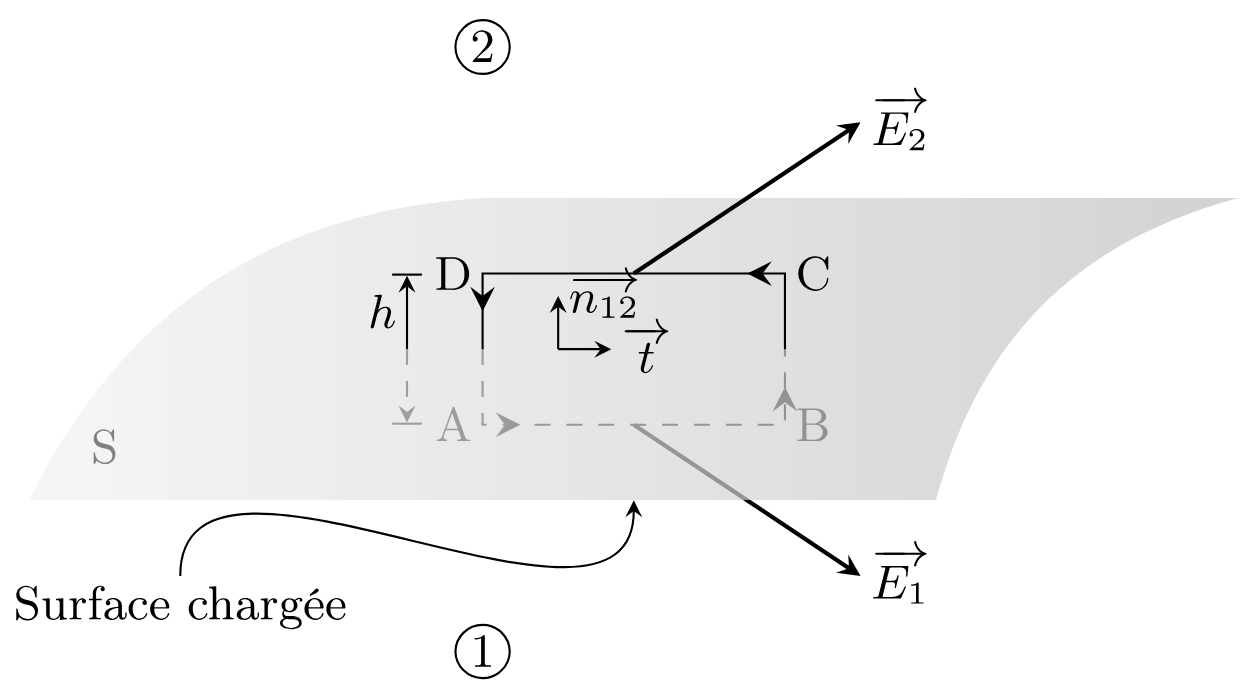
\includegraphics[width=0.36\linewidth]{passage_E_tangentiel.png}
	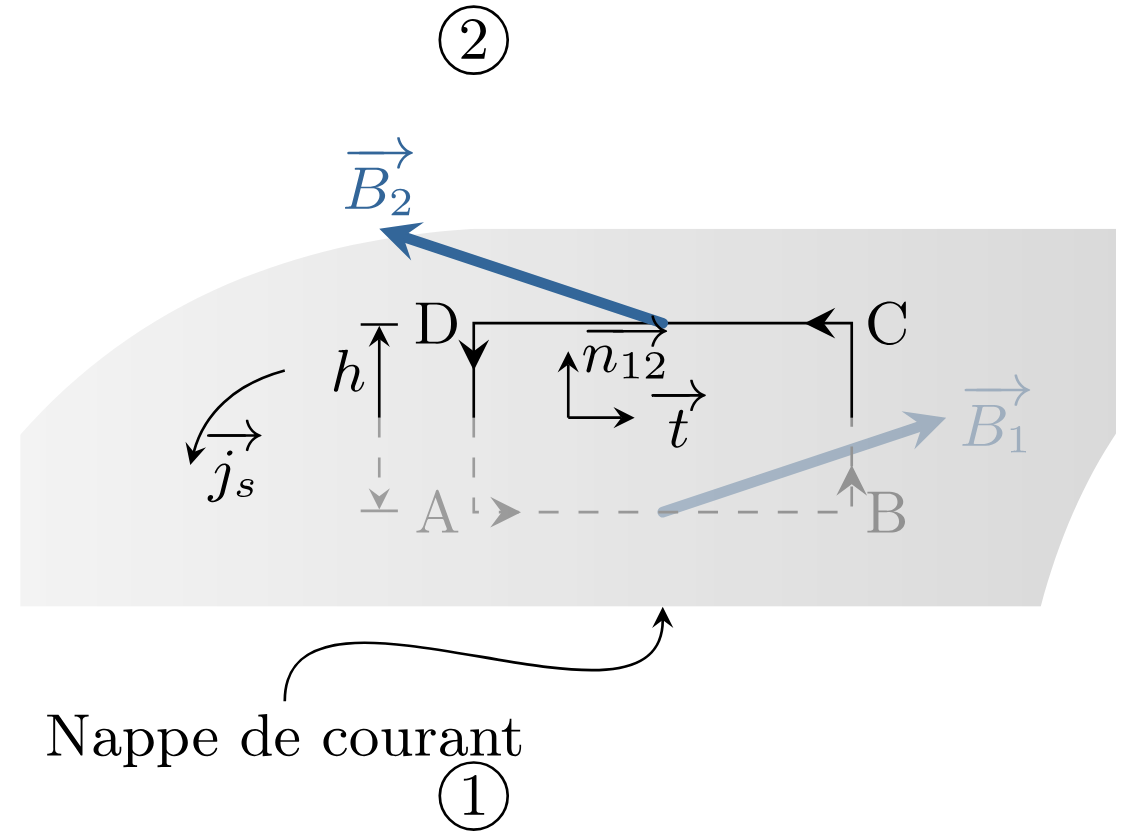
\includegraphics[width=0.27\linewidth]{passage_B_tangentiel.png}
	\caption{Surfaces et contours utilisés pour la démonstration des relations de passage concernant (de gauche à droite) la composante normale du champ électrique, la composante tangentielle du champ électrique, et la composante tangentielle du champ magnétique. Source : femto-physique.fr}
\end{figure}

\begin{demonstration}
	On considère un point $M$ situé à l'interface entre les deux milieux. Nous pouvons définir une base locale $(\vv n_{1 \to 2},\vv{t},\vv{u})$ telle que $\vv{t}$ et $\vv u$ sont tangents à l'interface et $(\vv n_{1 \to 2}, \vv t, \vv u)$ forme une base orthonormée directe.	

	Commençons par étudier la relation de passage pour la composante normale du champ électrique. On définit un volume élémentaire $\dd V$ constitué de deux éléments de surface $\dd S$ situés juste de part et d'autre de l'interface au niveau du point $M$ (sur le schéma, on a $S_0 = S_1 = S_2 = \dd S$). On applique le théorème de Gauss à ce volume, le flux du champ électrique sortant du volume est :
	\begin{equation}
		\oiint_{\dd V} \vv E \cdot \vv{\dd S} = (E_2 - E_1) \dd S 
	\end{equation}
	Par ailleurs la charge intérieure au volume est $\dd Q_{\rm int} = \sigma \dd S$. Nous pouvons en déduire que :
	\begin{equation}
		(E_2 - E_1)\cdot \vv n_{1 \to 2}  = \frac{\sigma}{\epsilon_0}
	\end{equation}

	Concernant la composante tangentielle du champ électrique, nous définissons un contour élémentaire $\dd \Gamma$ dans le plan $(M,\vv n_{1 \to 2}, \vv t)$ constitué de deux segments élémentaires de longueur $\dd \ell$ situés juste de part et d'autre de l'interface, et orientés respectivement selon $+\vv t$ dans le milieu 2 et selon $-\vv t$ dans le milieu 1. Les deux segments étant situés juste de part et d'autre de l'interface, la surface $\dd S$ délimitée par le contour est nulle. Nous pouvons alors utiliser la forme intégrale de l'équation de Maxwell-Faraday, en remarquant que le flux du champ magnétique à travers une surface nulle est également nul :
	\begin{equation}
		\oint \vv E \cdot \vv{\dd \ell} = - \frac{\dd}{\dd t} \iint_{\dd S} \vv B \cdot \vv{\dd S} = 0
	\end{equation}
	Nous en déduisons directement, en développant l'expression de la circulation du champ électrique le long de $\dd \Gamma$, que :
	\begin{equation}
		(\vv E_2 - \vv E_1) \cdot \vv t = 0
	\end{equation}
	Un raisonnement similaire en considérant un contour dans le plan $(M, \vv n_{1 \to 2}, \vv u)$ permet de montrer que :
	\begin{equation}
		(\vv E_2 - \vv E_1) \cdot \vv u = 0
	\end{equation}
	Nous concluons ainsi que :
	\begin{equation}
		\vv E_2 - \vv E_1 = \frac{\sigma}{\epsilon_0} \vv n_{1 \to 2}
	\end{equation}

	Considérons le champ magnétique, nous appliquons la forme intégrale de l'équation de Maxwell-Thomson au volume $\dd V$ défini précédemment, nous obtenons alors :
	\begin{equation}
		(\vv B_2 - \vv B_1) \cdot \vv n_{1 \to 2} = 0
	\end{equation}
	Nous appliquons désormais la forme intégrale de l'équation de Maxwell-Ampère au contour $\dd \Gamma$ défini précédemment :
	\begin{equation}
		\oint_{\dd \Gamma} \vv B \cdot \vv{\dd \ell} = \mu_0 I_{\rm enlace} + \frac{1}{c^2} \frac{\dd}{\dd t} \iint_{\dd S} \vv E \cdot \vv{\dd S}
	\end{equation}
	Le courant enlacé par le contour vaut $\dd I_{\rm enlace} = \vv{j_s} \cdot \vv u \dd \ell$, et le flux du champ électrique à travers la surface $\dd S$ est nul puisque cette surface est nulle. Nous en déduisons que :
	\begin{equation}
		(\vv B_2 - \vv B_1) \cdot \vv t = \mu_0 \vv{j_s} \cdot \vv u
	\end{equation}
	Nous pouvons également facilement montrer que :
	\begin{equation}
		(\vv B_2 - \vv B_1) \cdot \vv u = -\mu_0 \vv{j_s} \cdot \vv t
	\end{equation}
	Ce qui nous montre que :
	\begin{equation}
		\vv B_2 - \vv B_1 = \mu_0 \vv{j_s} \wedge \vv n_{1 \to 2}
	\end{equation}
	Ainsi, à partir des quatre équations de Maxwell, nous avons démontré les relations de passage du champ électromagnétique.
\end{demonstration}

\section{Réflexion sur un conducteur parfait}

On peut maintenant étudier le cas plus particulier de la réflexion sur un conducteur parfait, qui est une situation courante en pratique. On considère donc qu'une onde incidente se propage vers un conducteur en incidence normale, et donne naissance à une onde réfléchie. 
\begin{capex}
	Déterminer l'expression de l'onde réfléchie en fonction de l'onde incidente à partir des relations de passage. Quelle est le coefficient de réflexion en énergie ? En déduire que la puissance dissipée dans le conducteur parfait est nulle.
\end{capex}

Nous obtenons la propriété suivante :
\begin{proposition}
	Lors d'une réflexion sur un conducteur parfait, la totalité de l'énergie est réfléchie et un déphasage de $\pi$ est ajouté à l'onde (ce qui correspond à un coefficient de réflexion de -1 en amplitude) :
	\begin{equation}
		\vv E_r = E_0 \cos(\omega t + k z) \vv{e_x}
	\end{equation}
\end{proposition}

\begin{remark}
	Le même exercice peut être fait en prenant un conducteur non parfait : à partir des expressions des champs électrique et magnétique pour l'effet de peau, on peut calculer le vecteur de Poynting $\vv \Pi$ dans le conducteur et montrer que la totalité de l'énergie entrant dans le condcuteur est dissipée par effet Joule.
\end{remark}

\subsection{Quantité de mouvement du champ électromagnétique}

\textit{Cette partie n'est pas explicitement au programme de MP mais tombe régulièrement aux concours. Il n'est pas nécessaire d'apprendre le raisonnement par coeur mais il est bon de savoir le refaire.}

Nous pouvons utiliser l'exemple de la réflexion sur un conducteur parfait pour étudier la quantité de mouvement du champ électromagnétique. Nous pouvons calculer le champ magnétique associé à l'onde incidente et à l'onde réfléchie à l'aide de la relation de structure valide dans le vide, $\vv B = \frac{\vv u \wedge \vv E}{c}$, et ainsi nous obtenons :
\begin{align}
	\vv B_i = \frac{E_0}{c} \cos(\omega t - k z) \vv{e_y} \\
	\vv B_r = \frac{E_0}{c} \cos(\omega t + k z) \vv{e_y}
\end{align}
Au niveau de l'interface, les deux champs s'ajoutent (contrairement au champ électrique), et on a donc un maximum local (un "ventre") de champ magnétique :
\begin{equation}
	\vv B(z=0^-) = \frac{2 E_0}{c} \cos(\omega t) \vv{e_y}
\end{equation}
Par ailleurs, dans le conducteur parfait le champ magnétique est nul. Il y a donc une discontinuité de champ magnétique à l'interface, et par la relation de passage ceci va faire apparaître un courant surfacique $\vv{j_s}$ tel que :
\begin{equation}
	\vv B(z=0^+) - \vv B(z=0^-) = \mu_0 \vv{j_s} \wedge \vv{e_z} = -\frac{2 E_0}{c} \cos(\omega t) \vv{e_y}
\end{equation}
Nous en déduisons que :
\begin{equation}
	\vv{j_s} = \frac{2 E_0}{\mu_0 c} \cos(\omega t) \vv{e_x}
\end{equation}
Ce courant surfacique étant soumis à un champ magnétique non nul, une force surfacique va s'appliquer sur le conducteur, donnée par :
\begin{equation}
	\vv f_s = \vv{j_s} \wedge \frac{1}{2} (\vv B(z=0^+)+\vv B(z=0^-)) = \frac{2 E_0^2}{\mu_0 c^2} \cos(\omega t)^2 \vv{e_z}
\end{equation}
Nous pouvons alors remarquer que la force fait intervenir la densité volumique d'énergie électromagnétique que nous avons déjà calculé pour une onde plane progressive harmonique :
\begin{equation}
	u_{\rm em} = \epsilon_0 E_0^2 \cos(\omega t)^2
\end{equation}
si bien que la force surfacique, orientée selon $\vv{e_z}$, est assimilable à une force de pression sur le conducteur, appelée pression de radiation, et qui vaut :
\begin{equation}
	p = 2 u
\end{equation}
Cette propriété ne peut s'expliquer que si le champ électromagnétique présente une quantité de mouvement : l'onde électromagnétique incidente a une quantité de mouvement orientée selon $+ \vv{e_z}$ et l'onde réfléchie selon $-\vv{e_z}$. La réflexion de l'onde sur le conducteur implique une variation de quantité de mouvement qui est causée par la force exercée par le conducteur sur l'onde électromagnétique (principe d'action-réaction). 

Le fait que l'onde ait une quantité de mouvement non nulle s'interprète plus facilement dans le cadre du modèle corpusculaire de la lumière : on peut décrire les ondes électromagnétiques comme des ensembles de photons, transportant un quantum d'énergie $E = h \nu$ et une quantité de mouvement $\vv p$ à déterminer.
\begin{capex}
	Faire un bilan de quantité de mouvement sur les photons arrivant et quittant l'interface pendant $\dd t$. En déduire la valeur de la quantité de mouvement d'un photon.
\end{capex}

Nous obtenons la propriété suivante :
\begin{proposition}[Quantité de mouvement du champ électromagnétique]
	Le champ électromagnétique porte une quantité de mouvement, reliée au vecteur d'onde de l'onde. Un photon de vecteur d'onde $\vv k$ transporte la quantité de mouvement :
	\begin{equation}
		\vv p = \hbar \vv k
	\end{equation}
\end{proposition}


\subsection{Onde stationnaire}

On rappelle la définition d'une onde stationnaire :
\begin{definition}
	Une onde est dite stationnaire lorsque les variables de temps et d'espace sont découplées dans l'expression des champs associés à l'onde. Un champ $s(\vv x,t)$ correspondant à une onde stationnaire s'écrira ainsi $s(x,t) = f(x) g(t)$.

	On appelle noeuds les positions pour lesquelles $f(x) = 0$ (on n'a alors pas d'oscillations) et ventres les positions pour lesquelles $|f(x)|$ est maximal (oscillations d'amplitude maximale).
\end{definition}

\begin{capex}
	Montrer que la superposition de l'onde incidente et de l'onde réfléchie est une onde stationnaire.
\end{capex}


\section{Cavité à une dimension}

Dans de nombreux dispositifs physiques, on utilise une onde électromagnétique confinée entre deux plans conducteurs. L'onde est réfléchie par chacun des deux plans ce qui crée une cavité résonante. Dans le cas où une faible excitation existe entre les plans, ou bien un milieu amplificateur (c'est le cas notamment dans un laser), une onde stationnaire se forme entre les deux plans conducteurs.

\begin{figure}[htbp]
	\centering 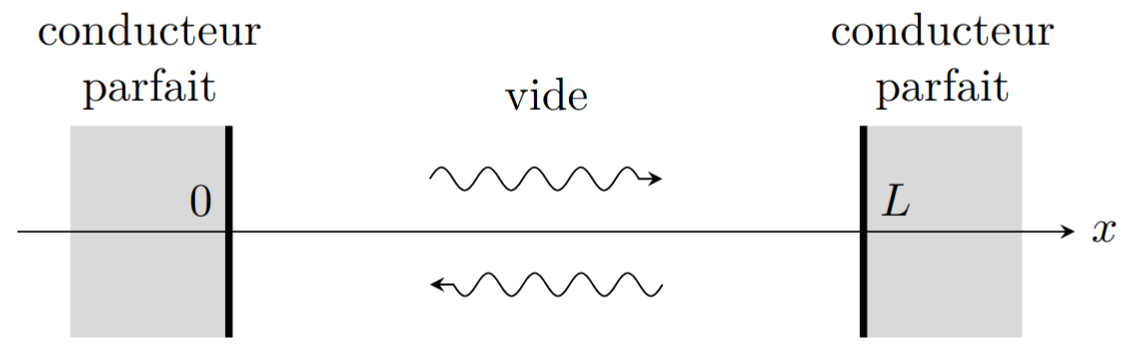
\includegraphics[width=0.6\linewidth]{cavite.png}
	\caption{Cavité électromagnétique entre deux conducteurs parfaits. Source : poly de cours de Etienne Thibierge.}
\end{figure}

\begin{capex}
	On considère deux conducteurs parfaits occupant les plans $z=0$ et $z=L$ et séparés par de l'air assimilé à du vide. On étudie une onde électromagnétique entre ces deux plans conducteurs, et on supposera toutes les quantités invariantes par translation selon $\vv{e_x}$ et $\vv{e_y}$. Quelles sont les conditions aux limites sur le champ électrique aux extrémités de la cavité ? Montrer qu'une onde stationnaire peut se former, dont la longueur d'onde $\lambda$ est quantifiée.  
\end{capex}

On peut alors définir les modes propres de la cavité :
\begin{theorem}
	Le champ électromagnétique confiné dans une cavité de longueur $L$ composée de deux conducteurs parfaits à une dimension a un nombre d’onde quantifié. Les fréquences des ondes stationnaires sont des multiples d’une fréquence fondamentale $f_1 = \dfrac{c}{2L}$ :
	\begin{equation}
		f_n = \frac{n c}{2L}
	\end{equation}
Ces fréquences possibles sont appelées fréquences propres du système. Les solutions correspondantes sont appelés modes propres.
\end{theorem}


\begin{figure}[htbp]
	\centering 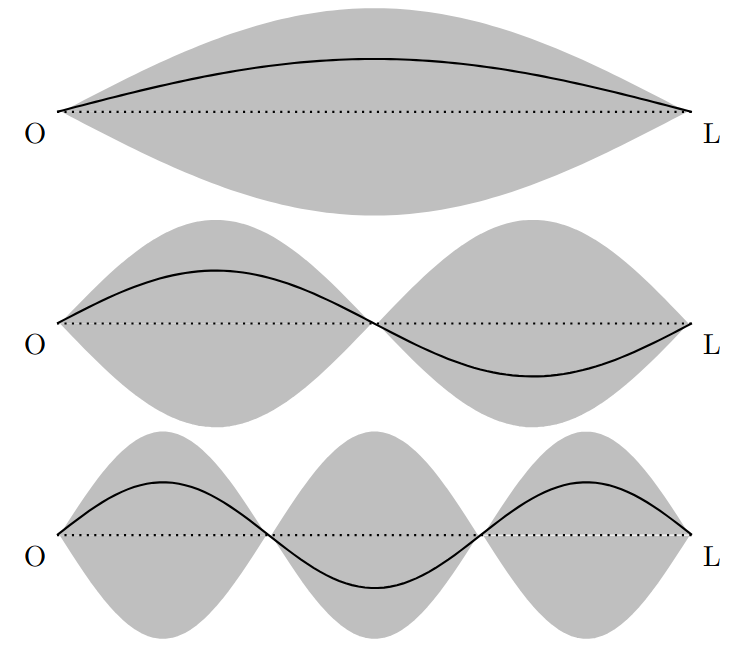
\includegraphics[width=0.5\linewidth]{modes_propres.png}
	\caption{Modes propres d'une cavité électromagnétique à une dimension. Source : poly de cours de Maxime Champion.}
\end{figure}

De manière générale, par principe de superposition, le champ électromagnétique est une combinaison linéaire de modes propres. Comme les modes propres sont des ondes stationnaires, leur vecteur de Poynting est nul et ils ne propagent pas d'énergie : l'énergie reste confinée dans la cavité.


\end{document}
